\documentclass[letterpaper,10pt,serif,draftclsnofoot,onecolumn,compsoc,titlepage]{IEEEtran}

\usepackage{graphicx}                                        
\usepackage{amssymb}                                         
\usepackage{amsmath}                                         
\usepackage{amsthm}                                          
\usepackage{cite}
\usepackage{alltt}                                           
\usepackage{float}
\usepackage{color}
\usepackage{url}
\usepackage{subfiles}
\usepackage{pdfpages}
\usepackage{blindtext}
%\usepackage[subpreambles=true]{standalone}
%\usepackage{import}
\usepackage{balance}
\usepackage[TABBOTCAP, tight]{subfigure}
\usepackage{enumitem}
\usepackage{array}
\usepackage{geometry}
\geometry{margin=.75in}
\usepackage{hyperref}
\usepackage{tikz}
\usetikzlibrary{shapes, positioning, calc}
%\usetikzlibrary{shapes, positioning, calc}
\usepackage{caption}
\usepackage{listings}
%\usepackage[utf8]{inputenc}
%pull in the necessary preamble matter for pygments output
\usepackage{pgfgantt}

\usepackage{graphicx}
\graphicspath{ {images/} }
\usepackage{tikz}
\usetikzlibrary{shapes.geometric, arrows}
\tikzstyle{startstop} = [rectangle, rounded corners, minimum width=3cm, minimum height=1cm,text centered, draw=black, fill=red!30]
\tikzstyle{io} = [trapezium, trapezium left angle=70, trapezium right angle=110, minimum width=3cm, minimum height=1cm, text centered, draw=black, fill=blue!30]
\tikzstyle{process} = [rectangle, minimum width=3cm, minimum height=1cm, text centered, draw=black, fill=orange!30]
\tikzstyle{decision} = [diamond, minimum width=3cm, minimum height=1cm, text centered, draw=black, fill=green!30]
\tikzstyle{arrow} = [thick,->,>=stealth]
\tikzstyle{process} = [rectangle, minimum width=3cm, minimum height=1cm, text centered, text width=3cm, draw=black, fill=orange!30]
% The following metadata will show up in the PDF properties
\hypersetup{
  colorlinks = false,
  urlcolor = black
  pdfpagemode = UseNone
}
%credit to %http://tex.stackexchange.com/questions/48152/dynamic-signature-date-line
\newcommand*{\SignatureAndDate}[1]{%
    \par\noindent\makebox[2.5in]{\hrulefill} \hfill\makebox[2.0in]{\hrulefill}%
    \par\noindent\makebox[2.5in][l]{#1}      \hfill\makebox[2.0in][l]{Date}%
}%

\parindent = 0.0 in
\parskip = 0.1 in
\title{STEM Academy Data Solution Final Report}
\author{Shannon Ernst, Kyle Nichols, Javier Franco\\ Group 48 \\ 13 June 2017 \\ CS 463 Spring 2017}
\begin{document}
\maketitle
\begin{abstract}
This document explores the development of the STEM Academy 
Data Solution during the 2016-2017 academic school year 
at Oregon State University. A web application to generate 
surveys and collect data was created to assist the 
STEM Academy in their data collection pursuits. 
\end{abstract}
\newpage
\tableofcontents
\newpage

\section{Introduction}
The STEM Academy program in Corvallis, Oregon, seeks to provide education in science, technology, engineering and math to the K-12 community through various programs, camps, and clubs.
They are self funded, relying on grants, donations and other sources, many of which require results-based data on the success of STEM Academy programs.
This data is collected from surveys that participants take while they are enrolled in one of STEM Academy's camps and other programs.
Currently, these surveys are administered on paper and the responses are tabulated by hand by volunteers.
This has not been an effective way of collecting current data to help secure funding and many of the surveys go untabulated.
The STEM Academy does have the ability to register participants online through Ideal Logic, but this does not help them with tabulating survey data.
They need a system which will allow them to electronically create surveys, a database to house all of the data from those surveys, and a report generation system so they can view the most current data in a timely and meaningful way.\\

A website which will allow the STEM Academy to create and distribute surveys, as well as view helpful data results, is the best solution.
The website should allow them to create questions that can be included across multiple surveys.
The questions should be able to be templated so that only one part of the question need change according to the topic of the survey.
Surveys should be able to be distributed via a web link or printed.
After a survey is taken, the data should be stored in a database according to the type of program.
This data should be queriable based on custom queries.
The user should be able to make a query based on the question and collected demographics as well as filter by program.
This service should be user friendly; the user should not need to know any SQL or other querying language in order to get data from the database.
After a query, the data should be able to be saved and added to a printable report so that it can actually be used in grant proposals and marketing material.
This website will be an all in one package for collecting and reporting on data in a timely fashion which is what the STEM Academy truly needs.\\

This project was worked on by Shannon Ernst, Kyle Nichols and Javier Franco.
Ernst focused on survey generation and management. 
Nichols focused on database management.
Franco focused on report generation.
Throughout the process the clients, STEM Academy, provided feedback on their needs but provided free reign on technical choices and implementation. \\

\section{Requirements Document}
\subsection{Original Document}
See next page. \\

\includepdf[pages={1-7}]{pdfs/requirements_document.pdf}
%\subfile{sections/requirements_document}
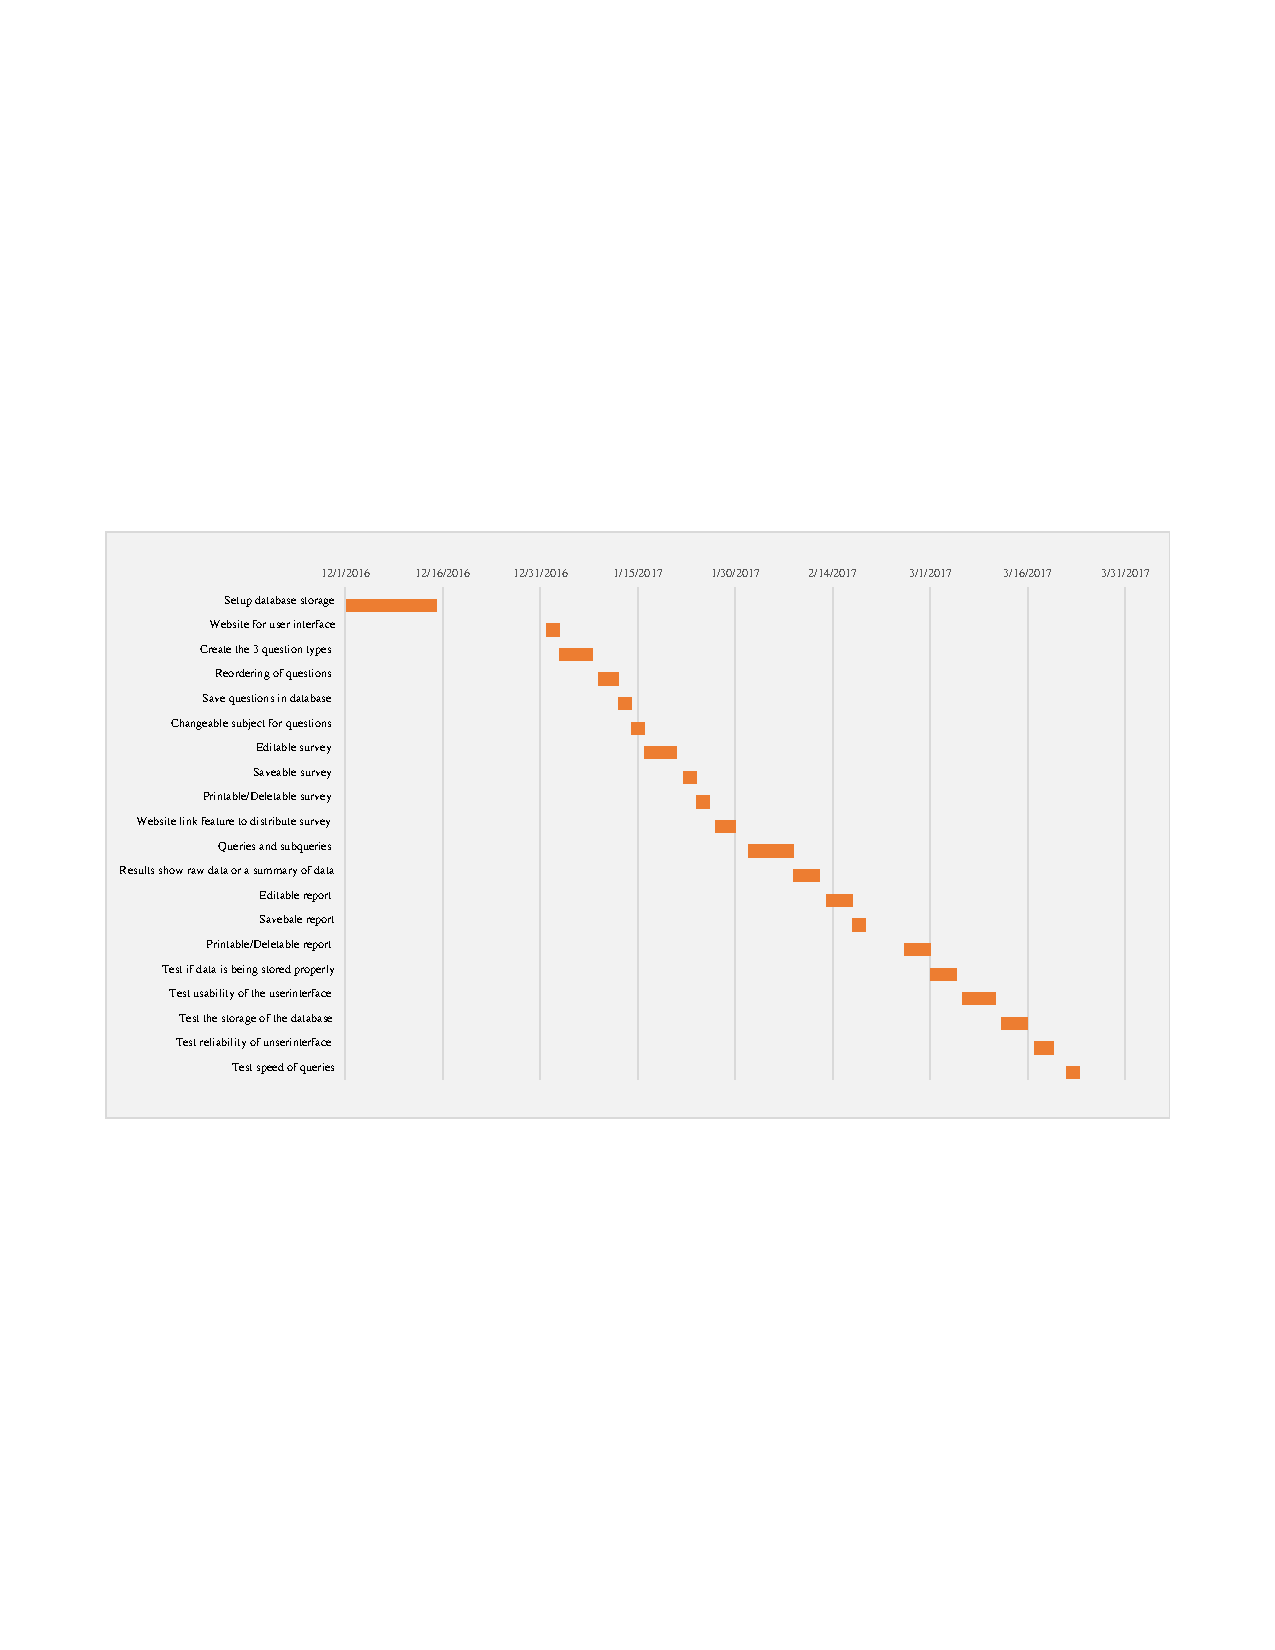
\includepdf[pages={1}]{pdfs/CS461Gantt.pdf}
\subsection{Changes to the Document}
There were no changes to the requirements document. 
\subsection{Gantt Chart Progression}
Our Gantt chart changed significantly over the course of 
the year. On the whole, things took a lot longer to implement 
than originally thought and we often had to circle back to 
fix issues. The updated chart is on the following page. \\
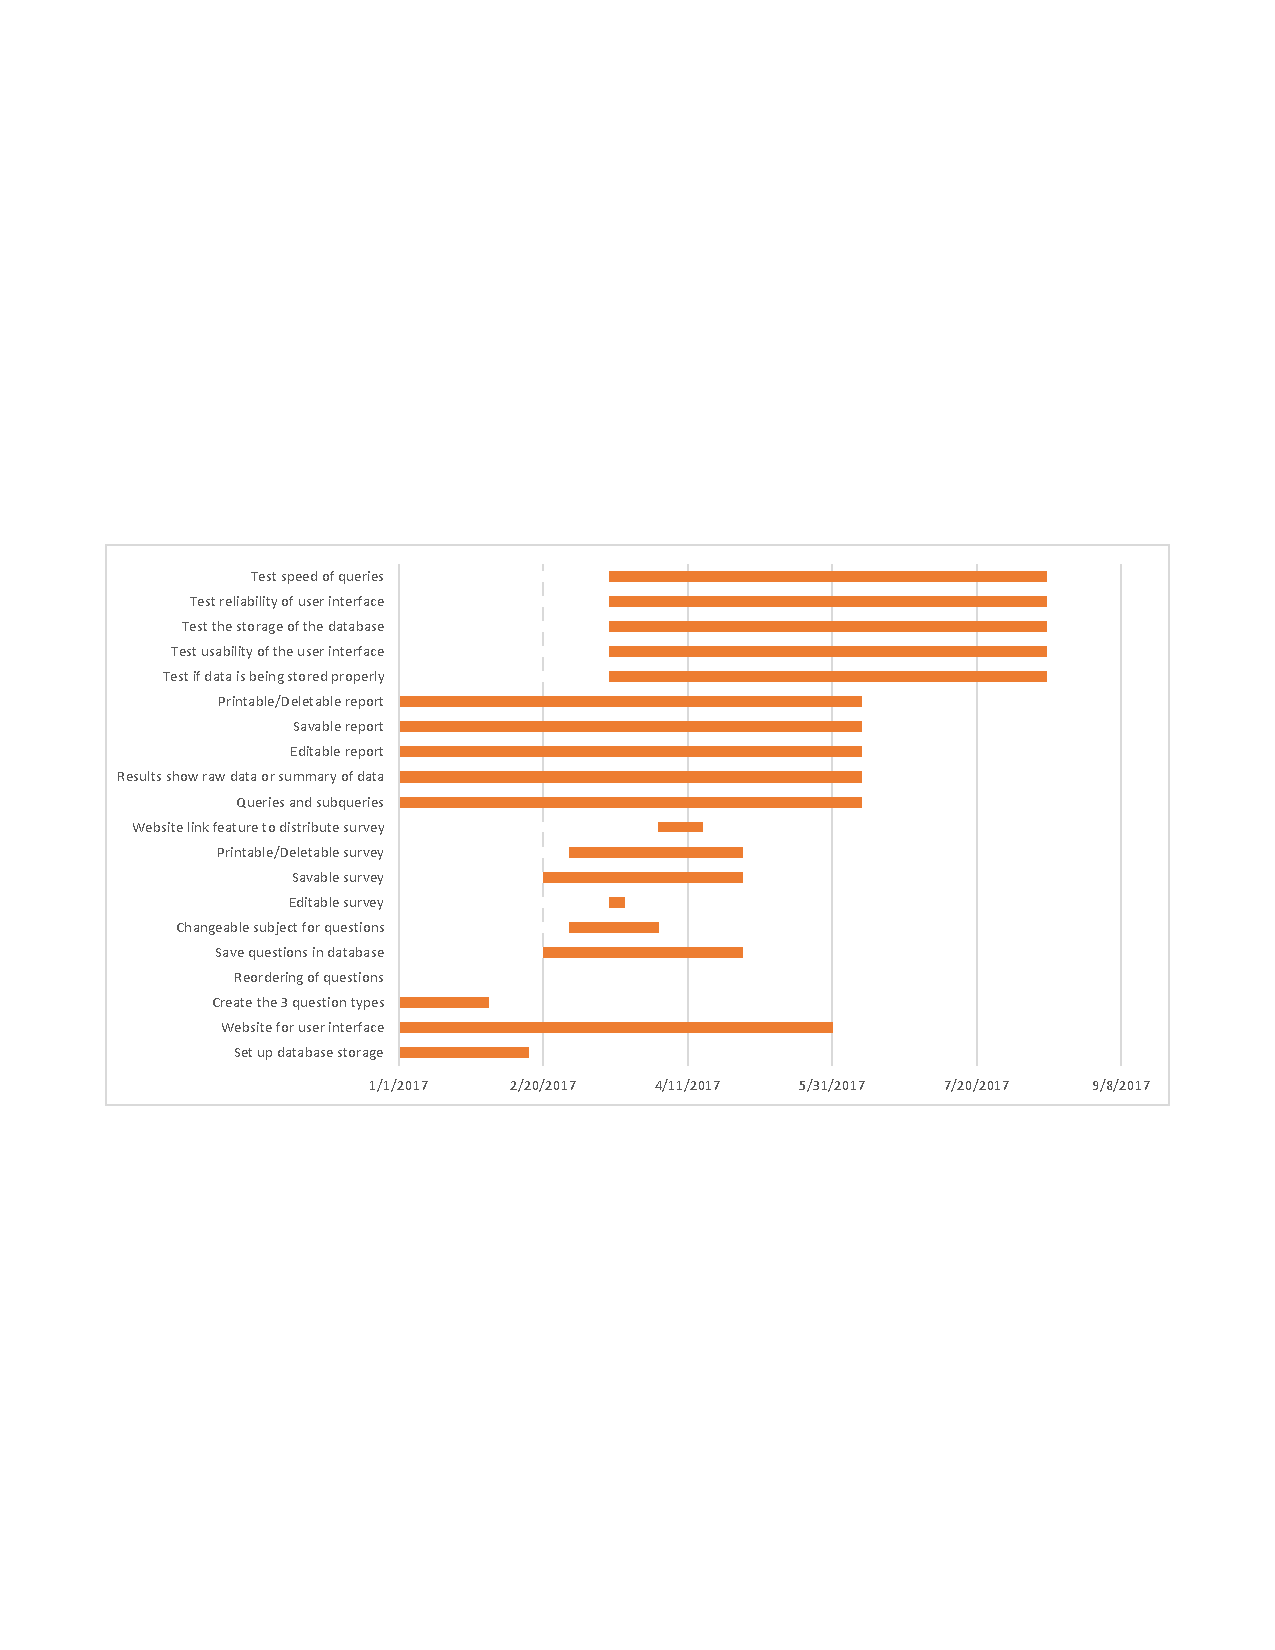
\includepdf[pages={1}]{pdfs/updated_gantt.pdf}

\section{Design Document}
\subsection{Original Document}
See next page. \\

\includepdf[pages={1-13}]{pdfs/design_doc.pdf}
\subsection{Changes to the Document}
\subfile{sections/design_changes}

\section{Technology Review Document}
\subsection{Original Document}
See next page. \\

\includepdf[pages={1-13}]{pdfs/fall_final_tech_review.pdf}
\subsection{Changes to the Document}
\subfile{sections/techreview_changes}

\section{Weekly Blogs Over the Year}
\subfile{sections/fall_weekly_blogs}
\subfile{sections/winter_weekly_blogs}
\subfile{sections/spring_weekly_blogs}

\section{Poster}
See next page. \\

\includepdf[pages={1}]{pdfs/Group48Poster_Draft2.pdf}
\section{Documentation}
The following sections describe how the STEM Academy Data Solution was implemented.
The first section will cover the overall structure and usage of the web service before delving more deeply into each component in its own section.
Currently, STEM Academy Data Solution is developed for the Google Chrome web browser.
Usage of the website through other browsers is not guaranteed to work correctly.
\subsection{Overall}
\subfile{sections/overall_doc}
\subsection{Survey Generation}
\subfile{sections/survey_generation_doc}
\subsection{Database}
\subfile{sections/database_doc}
\subsection{Report Generation}
\subfile{sections/report_generation_doc}

\section{Reflection}
\subsection{How to Learn}
For learning how to use new technology we did not use any books and we did not get outside help from other people that were not involved in our group.
We learned new technology by researching the things that we needed on the fly.
The majority of the things we needed were found in StackOverflow pages.
Another website was useful was w3schools for looking up how to use a CSS style sheet, HTML, and PHP.
This website was useful by providing code examples and also by generating the results of the code. 
Below is the order of usefulness of the websites:
1.StackOverflow
2.w3schools
\subsection{What was Learned}
\subfile{sections/learned_ernst}
\subfile{sections/learned_nichols}
\subfile{sections/learned_franco}

%\bibliographystyle{ieeetr}
%\bibliography{writing1}
\begin{appendices}
\subfile{sections/appendix}
\end{appendices}
\end{document}